\newcommand{\simulator}{simulator}

\begin{myblock1}{\Large PyNN : a common API for neuronal network modelling \phantom{\Huge $\beta$}}
    
	\vskip-10mm
	\begin{columns}[c]
		\column{.50\textwidth}
		\uncover<1->{
			\hspace{-8mm}
			\begin{itemize}
				\item[$\rhd$] facilitate model sharing and reuse
				\item[$\rhd$] simplify validation of simulation results
				\item[$\rhd$] provide a common platform on which to build other tools
				\item[$\rhd$] provide a more powerful API for neuronal network modelling
				\item[$\rhd$] hide complexity of parallelization from user
			\end{itemize}
		}
		\column{.45\textwidth} 
		\vskip30mm
		\only<1>{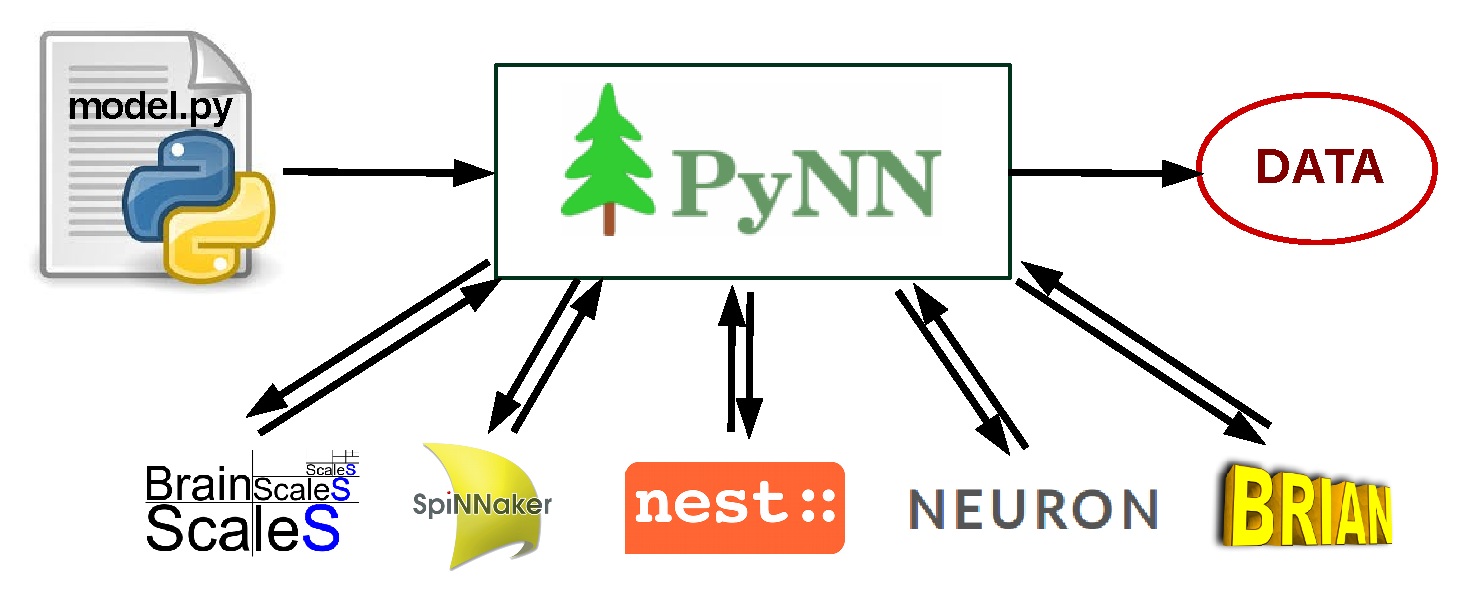
\includegraphics[width=0.99\textwidth,angle=00]{\imgpath/pynn.pdf}}
	\end{columns}
	\vspace{5mm}
	
	\begin{columns}[c]
		\column{.50\textwidth}
		\footnotesize
		\only<1>{\texttt{\textcolor{red}{import pyNN.nest as \simulator}}\newline}
		\only<1>{\texttt{\textcolor{red}{import pyNN.neuron as \simulator}}\newline}
		\only<1>{\texttt{\textcolor{red}{import pyNN.brian as \simulator}}\newline}
		\only<1>{\texttt{\textcolor{red}{import pyNN.brainscales as \simulator}}\newline}
		\only<1->{\texttt{\textcolor{red}{import pyNN.spiNNaker as \simulator}}\newline}
		            
		\texttt{cell\_type = \dots}\newline
		
		\only<1->{\texttt{p1 = \textcolor{red}{\simulator}.\textbf{Population(}size1, cell\_type, structure\textbf{)}}}\newline
		\only<1->{\texttt{p2 = \textcolor{red}{\simulator}.\textbf{Population(}size2, another\_cell\_type, structure\textbf{)}}}\newline
		            
		\only<1->{\texttt{all = p1 + p2}}\newline
		\only<1->{\texttt{all.record(["spikes", "v"])}}\newline
		            
		\only<1->{\texttt{connections = \textcolor{red}{\simulator}.\textbf{Projection(}p1, p2, connection\_rule, synapse\_type\textbf{)}}}\newline
		   
		\texttt{\textcolor{red}{\simulator}.run(1000.)}\newline
		            
		\column{.45\textwidth} 
		\vskip+6mm
		\normalsize
		% \fontsize{6}{9}\selectfont
		PyNN is a \textbf{simulator-independent language} for building spiking neuronal network models and provides a library of:
		\begin{itemize}
			\item$\rhd$ standard neuron, synapse and synaptic plasticity models
			\item$\rhd$ commonly-used connectivity algorithms \\[4mm]
		\end{itemize}
		The user is not restricted to the standard models and can also use any neuron or synapse model supported by your simulator.\\[24pt]
		            
		For downloads and full documentation see:\\[4pt]
		\centering{\texttt{\textbf{http://neuralensemble.org/PyNN/}}}
		\normalsize
		
	\end{columns}

\end{myblock1}